\documentclass{article}
\usepackage[utf8]{inputenc}
\usepackage{graphicx}

\title{Introduction to Machine Learning --- Notes}
\author{The ML Primes}

\usepackage{amsmath,amssymb}
\DeclareMathOperator{\E}{\mathbb{E}}

\newtheorem{theorem}{Theorem}[section]
\newtheorem{lemma}[theorem]{Lemma}
\newtheorem{proposition}[theorem]{Proposition}
\newtheorem{corollary}[theorem]{Corollary}

\newenvironment{proof}[1][Proof]{\begin{trivlist}
\item[\hskip \labelsep {\bfseries #1}]}{\end{trivlist}}
\newenvironment{definition}[1][Definition]{\begin{trivlist}
\item[\hskip \labelsep {\bfseries #1}]}{\end{trivlist}}
\newenvironment{example}[1][Example]{\begin{trivlist}
\item[\hskip \labelsep {\bfseries #1}]}{\end{trivlist}}
\newenvironment{remark}[1][Remark]{\begin{trivlist}
\item[\hskip \labelsep {\bfseries #1}]}{\end{trivlist}}

\newcommand{\qed}{\nobreak \ifvmode \relax \else
      \ifdim\lastskip<1.5em \hskip-\lastskip
      \hskip1.5em plus0em minus0.5em \fi \nobreak
      \vrule height0.75em width0.5em depth0.25em\fi}

\DeclareMathOperator*{\argmax}{arg\,max}
\DeclareMathOperator*{\argmin}{arg\,min}

\begin{document}

\maketitle

\setcounter{section}{-1}
\section{Course Content}
\begin{itemize}
    \item Classification algorithms
    \begin{itemize}
        \item Focus on Bayesian
        \item Overview of other \~1001 algorithms
    \end{itemize}
    \item Applications 
    \begin{itemize}
        \item Internet: spam, recommendation, adverts
        \item Other: Kinect, medical
    \end{itemize}
    \item General issues
    \begin{itemize}
        \item Why learning from examples is possible?
        \item Comparing learning algorithms
    \end{itemize}
\end{itemize}

    \subsection{A Quick Glossary}
        We use the term `rv' as short-hand for `Random Variable' and `PDF' to shorten `Probability Distribution Function'.

\section{Review of Probability Theory}
    \subsection{Central Limit Theorem}
        This can be seen when rolling $N$ number of dice and is defined as the distribution of their sum.
        \begin{definition}
        The sum of $N$ rvs with mean $m$ and standard deviation $s$ can be approximated by a normal distribution with mean $\mu=Nm$, and std $\sigma=\sqrt{Ns}$.
        \end{definition}
        
        The probability density of a normal distribution
        \begin{equation}
        f(x) = \frac{1}{\sqrt{2\pi}\sigma}\exp{-\frac{{(x-\mu)}^2}{2\sigma^2}}
        \end{equation}
    
    \subsection{Correlation}
        Correlation is measured as a value from -1 to 1 with the magnitude telling us to what degree the value of one rv implies the value of another one. A positive correlation is given to a relation where a positive value for one variable implies a positive value in the other, whilst a negative correlation is given for when a positive value in one implies a negative value in the other. No correlation signifies no discernible relation of any kind.\\
        \\
        More formally, the correlation, $r$, between variables $X$ and $Y$ is defined as
        \begin{equation}
            r = \frac{\textrm{cov}(X,Y)}{\sigma(X)\sigma(Y)}
        \end{equation}
        Where the Covariance is defined as
        \begin{equation}
            \textrm{cov}(X,Y) = \E((\underbrace{X-\E(X)}_\alpha)(Y-\E(Y))) = \E(XY)-\E(X)\E(Y)
        \end{equation}
        
        $\alpha$ is the difference between an instance of rv $X$ and $X$'s mean/expected value.
        
    \subsection{Conditional Probability}
        A conditional probability is the probability that an event will occur given that another event has known to occur. The probability of A given B is written as $P(A|B)$.
        
        \textbf{Example given in lectures}
        If the probability of having cancer is $c$ and the probability of smoking is $x$, then the probability of having cancer ($P(c|x)$) if you smoke is the number of smokers with cancer / the total number of smokers. Hence:
        \begin{equation}\label{equ:condprob}
            P(c|x) = \frac{P(c\wedge  x)}{P(x)}
        \end{equation}

    \subsection{Bayes' Rule}
    
    Sometimes know as Bayes' Theorem, Bayes' Law, etc. 
    
    Let $A$ and $B$ be a pair of events. Bayes' Rule states that
    
    \begin{equation}\label{equ:bayes_rule}
        P(A|B) = \frac{P(B|A)P(A)}{P(B)} 
    \end{equation}
    
    To say that this rule is important would be an understatement -- it is the entire basis of a Bayesian Classifier. If $B$ is a feature vector and A is a class, this rule allows us to find the probability that an instance belongs to a class, given that it exhibits the features in B. For classification, the denominators for each class are usually the same, so it suffices to calculate

    \begin{equation}
        P(A|B) \propto P(B|A)P(A) 
    \end{equation}
    

    \subsection{Independence}
        If two r.v. $A$, $B$, are independent then knowing about one gives us no better knowledge about the value of the other, hence $P(A|B)=P(A)$. Using Equation~\ref{equ:condprob}, we can say
        \begin{equation}
            P(A\wedge B)=P(A)P(B) 
        \end{equation}
        
    \subsection{Independence vs Uncorrelated}
        Independence and uncorrelated are different. Correlation is a linear dependency, where as dependence is broader relationship\footnote{My description above doesn't really say this.}. Independence implies uncorrelated but the reverse is not true. Correlation implies dependence, but again the reverse not true.
        
    \subsection{Bayesian Belief Networks}
        % git could be used to model a Bayesian belief network. Just sayin'
        Bayesian belief networks extend the Bayesian classifier model by allowing dependencies between attributes, for when assuming class-conditional independence between features just doesn't cut the mustard. Let us look at Rafal's example from the slides:
        \begin{figure}[h]
            \centering
            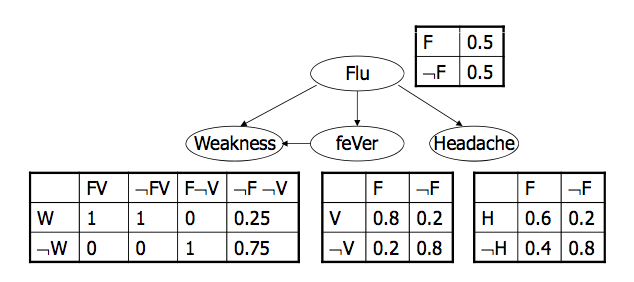
\includegraphics[scale=0.5]{images/slidebbn.png}
            \caption{Raffa's Graph}
        \end{figure}
        The trick here is that belief networks are displayed as directed acyclic graphs, typically shown with the classes at the top. In Rafal's example, there are only two classes Flu (F) and Not Flu, so he only needs the one node to represent it. He has three attributes, feeling weak (W), running a fever (V) and having a headache (H).
        In these graphs, the direction of an edge between nodes indicates the implied relationship between the two. I.e
        
        $$A\rightarrow B$$
    
    Means that B is more likely given A. It is not necessarily a causal relationship. As you can see in the tables Raffa provides, he has calculated the conditional probability for each attribute as a function of BOTH of its parents. This is the key thing here; these values are what we use in the new version of the argmax comparison. On Rafal's next slide he does some mathematical jiggery-pokery but the bottom line is simple. Instead of attributes being conditional only on the class, they are now conditional on all parents in the graph. Simples.
    
    In a normal classifier we simply multiply the conditional probabilities of each attribute given a class, but now we multiply the conditionals given all parents of that attribute. It is actually quite a simple extra step, reflected in the two examples below; rather than the current straight multiplication of \emph{attribute | class}, each P term becomes a product of \emph{attribute | parents}.
    $$
        c(x) = arg max \big(P(a_{1}...a_{n} | c_{i})*P(c_{i})\big) = argmax P(a_{1}...a_{n},c_{i})
    $$
    $$
        \Rightarrow P(a_{1}...a_{n},c_{i}) = \prod_{x = 1}^{n}\big(P(a_{x} | Parents(a_{x}))*P(c_{i})\big)
    $$
    We are simply adding a handful of additional multiplications in exchange for a fair approximation of inter-attribute dependencies.
    
\section{General Classifier Terminology}
    \subsection{Margin}
        The margin of a classifier is simply the smallest distance between its separating boundary and the closest instance. Different kinds of classifiers tend to produce different styles of boundary:       
        \begin{itemize}
            \item Tree and rule based classifiers will always divide sets parallel to the axes.
        
            \item Bayesian classifiers give a smoother but still linear divide.
        
            \item Lazy classifiers (think nearest neighbour) give a jagged divide composed of many straight lines around instances.
        
            \item Meta and function classifiers give the smoothest divide.
        \end{itemize}
    \subsection{Meta Learning}
        So named because it is a classifier built of many classifiers. One example is a \textbf{bagging algorithm}, which simply takes the mean separation boundary of several classifiers, each of which is trained on a different subset of the training set. Related to Boosting, which we'll cover in a jiffy.
        
    \subsection{Bias and Variance}
        Different classifiers tend to have different biases and variances, and classifier design choices are usually about finding a trade-off between the two.
        
        The `Bias' of a classifier indicates a propensity for the classifier to favour a particular class. Imagine we have three classes, \emph{Orange, Lemon and Grapefruit}. If our classifier, no matter what training data we use, consistently gets all the grapefruits right, but also classifies half of the oranges and half of the lemons as grapefruits then this is an example of bias towards the class of grapefruits. Mmmmm grapefruit.
        
        The `Variance' of a classifier is the opposite problem; say we have the same three classes, and a new classifier, whom I shall call Bob. We also have 3 different but equally good training sets for Bob. Say we train Bob on each of these sets and then ask him to classify an orange. If he gives us a different answer every time, then Bob has a high variance; he is highly dependent on his training data matching his test data in order to be of any use.
        
    \subsection{Explanation}
        
        As a rule of thumb, the more geometric the dividing line is, the more explanation is retained as to why an item is classified as it is. For instance in a decision tree we can exactly see why an item was classified the way it was based on the decisions made. In a function based classifier this is not so trivial, and in complex classifiers like large Neural Networks it can be almost impossible to do by inspection.

    \subsection{Boosting}
        Boosting allows us to easily form a strong classifier from a large number of weak classifiers. This is done by adjusting the weighting of training data over a series of iterations, reducing the overall error. It is best explained as a process of steps, so I shall. While its doubtful you need to remember the exact equations I have included them just in case. Imagine a booster, which runs over $T$ iterations,
        
        \begin{enumerate}
            \item Initialise the weight of every training item to $\frac{1}{m}$
            \item Create a new weak learner, $h_t$
            \item Train this learner on the weighted data to minimise its error\footnote{This simply means, train each classifier this one is made up of, with the weighted data. E.g. in a Bayesian filter we can weight a word by pretending there are more occurences than there are.}, $E_t$.
            \item Computer the importance of this meta-classifier with the formula:
                $$ \alpha_t = \frac{1}{2} \ln{\left (\frac{1-E_t}{E_t}\right )}$$
            \item \textbf{Increase} the weights of \textbf{incorrectly} classified items.
            \item \textbf{Decrease} the weights of \textbf{correctly} classified items.
            \item If $t < T$ GOTO 2.
            \item Our actual classification is now calculated as the sum of each weighted classifier:
                $$ H(x) = \sum\limits_{t=1}^T \alpha_t h_t(x) $$
        \end{enumerate}
        
    \subsection{Accuracy}
        \subsubsection{p-value}
            p-value is the probability of observing data at least as extreme as that observed, given that the null hypothesis is true. In simple terms, it relates to a percentage of results in a t-test that satisfy a criterion. Read on, dear student...
            
        \subsubsection{T-test}
            T-tests are really very simple, and are not to be feared! The idea is straightforward; we have our set of results from our first classifier (C1). This set forms a distribution of sorts, which we just model as a normal/Gaussian distribution with a mean and std. deviation. We then have another set of results from classifier number 2 (C2), which show a small improvement in accuracy! ``HOORAY'', I hear you cry, ``Victory is ours'', but then the shadowy figure of Raffa looms over and says `T-Test it at the p = 0.05 significance level'. What to do?
            
            Well, we pick our hypothesis that we are testing to be simply that C2 is better than C1 at the significance level p = 0.05. This means, in plain talk, that if we were to generate random samples from C1's original distribution, and take their mean value, only 5\% of the time (or less) would those means be greater than or equal the mean of C2's distribution.
            
            All you do is this: pick a number of tests to run, say 10000; We shall call this number $ITERS$. Create a counter $p$ that is initialised to 0. Then for each test you take a bunch of random samples based on C1's distribution (the exact number should be the same as the number of original samples that formed the distribution). If the mean of these new samples is greater than or equal to the mean of C2's distribution, you add 1 to $p$. At the end, you divide $p$ by $iters$, and if this number is greater than your significance level you fail the test. That is a straight-up, one-sided paired t-test.
            
            We only ever use paired t-tests when comparing classifiers, because a `paired' test is one that is run on the same test data. Comparing results from different data sets uses unpaired t-tests which are more complicated and not covered in the course.
            
    \subsection{VC Dimension}
        The VC dimension is the size of the largest set of instances that a classifier can `shatter'. It can do this iff \textbf{for every class labelling} of the instances, there exist parameters of the classifier for which \textbf{all instances are labelled correctly}.
        % I believe the following is true
        Such a condition can generally be tested by training on the same set that we test on, no cross validation or nothing. 
        
        The larger the VC dimension of a classifier, the larger bound on error we can expect between training and test data. This is textbook Occam's Razor. For example with a K-nearest neighbour algorithm with $K=1$, when tested on the training data, the VC dimension is infinity, since the nearest neighbour in the training data is at exactly the point we are on. However, its obvious that in practice this classifier would be pretty... \emph{shit}.
        
        In general, increasing the VC dimension will lower test-data errors at first, then increase the error as overfitting to the training data occurs.
        
        Also, VC stands for Vapnik–Chervonenkis. Hopefully there will not be any marks for spelling that correctly.
            
\section{The Na\"{i}ve Bayes Classifier in Spam Filtering}

    We assume that every word in an email appears independently from all others, and that the ordering of words is irrelevant. We define a vocabulary, $W$, the set of all words that appear in the training data, and our two classes will be called $H$ and $S$ for Ham and Spam respectively. To train a Na\"{i}ve Bayes Classifier, we must estimate each of the following;
    
    \begin{align*}
        P(H) &\mbox{ -- the probability of receiving a Ham email}\\
        P(S) &\mbox{ -- the probability of receiving a Spam email}\\
        P(w | H) &\mbox{ -- the probability that a Ham email contains $w$, for each $w \in W$}\\
        P(w | S) &\mbox{ -- the probability that a Spam email contains $w$, for each $w \in W$}
    \end{align*}

    Using Bayes' Rule -- eqn \ref{equ:bayes_rule} -- we can then classify an unseen email containing words $w_1, w_2, w_3,...w_n$ by calculating $P(H|w_1,...,w_n)$ and $P(S|w_1,...,w_n)$ as follows;
    
    \begin{align*}
        P(H|w_1,w_2,....w_n) &\propto P(H)\prod^{n}_{i=1}P(w_i|H) \\
        P(S|w_1,w_2,....w_n) &\propto P(S)\prod^{n}_{i=1}P(w_i|S)
    \end{align*} %Holy dicks this LaTeX compiler screws up some of these symbols pretty well...

    We can then classify the unseen email as whichever of the two classes is more likely. For practical cases, it is usually preferred to calculate and compare the logarithms of each of these values, since the probabilities can quickly become very small.
    
    When estimating probabilities, it is common to apply the Laplace correction to avoid probabilities of 0 or 1. The Laplace Correction is analogous to adding two emails to both the Spam and Ham training sets -- one containing every word, and one containing no words, so the estimated probabilities become;
    
    \begin{align*}
        P(w | H) &= \frac{\mbox{number of $w$s in Hams} + 1}{\mbox{number of words in all Hams} + \mbox{number of known words}}\\
        &\\
        P(w | S) &= \frac{\mbox{number of $w$s in Spams} + 1}{\mbox{number of words in all Spams} + \mbox{number of known words}}\\
    \end{align*}

    This correction is usually fairly important, since it is not uncommon to observe words that appear only in Spam emails, or words that appear only in Ham emails. A similar but less important correction can also be applied to $P(H)$ and $P(S)$, resulting in the estimates;
    
    \begin{align*}
        P(H) &= \frac{\mbox{number of Hams}+1}{\mbox{number of emails}+2}\\
        & \\
        P(S) &= \frac{\mbox{number of Spams}+1}{\mbox{number of emails}+2}
    \end{align*}

    Making these corrections is not always necessary, check what corrections are called for on each question to maximise marks! It is also important to note that when using belief networks and applying Laplace correction we must apply additional correction for each attribute that has multiple parents, to make sure that every combination of parents is present at least once in the calculated probability.
%      ____                     _____________         _____________
% ____//_]|________        ____//__][__][___|    ____//__][______||
%(o _ |  -|   _  o|       (o  _|  -|     _ o|   (o _ |  -|   _   o|
% `(_)-------(_)--'        `-(_)--------(_)-'    `(_)-------(_)---'
%  ______________     ________________        __________________
% //__][__\\____\\   //__][__\\___\\__\      |[B][E][S][S][E][Y]|
%(o _-|         o|  <o  _||  -|   _  o|      |o _         _  _  |
% `(_)-------(_)-'   `-(_)-------(_)--'       `(_)-------(_)(_)-"
%      ____________             ______              ______
% ____//__][__\\___\       ____//__][_\      ______//__][_\__
%(o _ |  -|   _   o|      [o _ |  -| _ \    /o _   |  -| _   \
% `(_)-------(_)---'       `(_)-----(_)-'   `-(_)-------(_)---'
%      ________              _____                  _
% ____//__][__\\___     ____//__]|              ___//]    ____
%(o _ |  -|   _  o|    (o _ |   -|_________    |o_   '---' _ |
% `(_)-------(_)--'     `(_)-------(_)(_)--'   `(_)-------(_)''
%      _                     ______________               _
% ____//]_________      ____//__]| ymbirtt|        ______//________
%(o _ |  -|  _  o|     (o _ |   -|  _  _  |       /o _   |  -| _   \
% `(_)------(_)--'      `(_)-----'-(_)(_)-'       `-(_)-------(_)---'
    
    % Because who doesn't like ASCII cars in source?
    
\section{Ad Recommendations}

    \emph{Hello reader, if you don't understand the difference between probability and probability density, this section will get rather sticky. Rafal's notation in this area is utterly terrible, using $P$ to mean both. If you do not know what a probability density function is for, go to wikipedia, look it up, and then read this chapter afterwards.}

    Let $X \sim Bern(\mu)$, that is X is a Bernoulli random variable with $P(X=1) = \mu$, $P(X=0) = 1-\mu$. $\mu$ is an unknown parameter, and in this problem, X is an indicator for the user clicking on the advert that we shove in his face. We'd like to estimate $\mu$, which represents the relevance of this advert to a particular type of user. We do this by modelling $\mu$ itself as a random variable.
    
    To reiterate, $P(X=1)=\mu$, and $\mu$ is a random variable. This sounds nasty, but isn't too bad. We will iteratively reduce the variance of $\mu$ until it hits 0, at which point we will know its value.
    
    Initially, we have no information about $\mu$, so we assume $\mu \sim U(0,1)$, ie $\mu$ is uniformly distributed between 0 and 1, $\mu$ has density $f_\mu(m) = 1$ for $m \in [0,1]$. The rule by which we refine $\mu$ is simple;
    
    \begin{equation}
        f_\mu(m) \propto m^s(1-m)^f \quad \footnote{It seems as though the normalisation constant isn't examinable, but if you're interested it's $\beta(s,f)^{-1} := \frac{(s+f-1)!}{(s-1)!(f-1)!}$}
    \end{equation}

    Where $s$ is the number of successes -- times the advert is clicked -- and $f$ is the number of failures -- times the advert is displayed but not clicked. As this is repeated, the variance decreases, and we eventually reach a constant for $\mu$.
    
    For example, if the advert is displayed once and clicked once, $f_\mu(m) \propto m^1(1-m)^0$. If the advert is displayed twice, clicked once, and ignored once, $f_\mu(m) \propto m^1(1-m)^1$. If the advert is displayed 20 times, clicked 14 times, and ignored 6 times, $f_\mu(m) \propto m^{14}(1-m)^6$. This evolution is displayed below, though this image is taken from Rafal's slides in which P refers to $f_m$:
    
    \begin{center}
        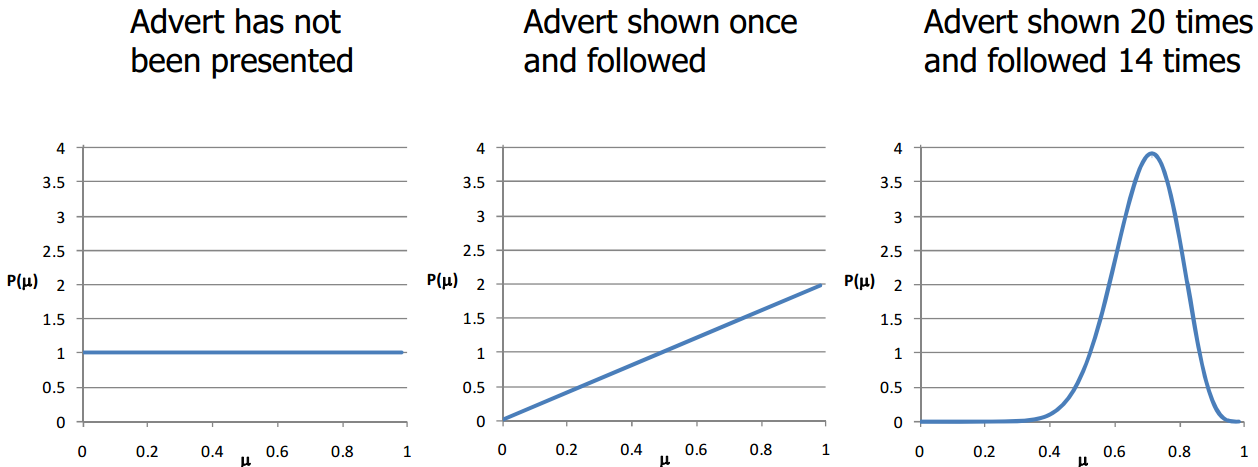
\includegraphics[width=\textwidth]{images/mu-graph.png}
    \end{center}
    
    When asked in an exam, you're generally expected to be able to plug these values into the formula, and explain what the balls is going on with them, though this document is by no means a crystal ball.
%%%%%%%%%%%%%%%%%%%%%%%%%%%%%%%%%%%%%%%%%%%%%
% 'sup Matt. I've gone and rewritten a significant amount of your section. If this is terrible in some way, come chat with me and we'll work something out.
%%%%%%%%%%%%%%%%%%%%%%%%%%%%%%%%%%%%%%%%%%%%%

%    If an advert is shown 3000 times, and clicked 1000 times, and another is shown 3 times, and clicked once, they will have an equal $P(x)=0.33$. However, this does not tell the full story, intuitively we know that we can have more confidence in the advert shown 1000x more than the other.
    
%    Confidence in machine learning describes the probability \textbf{distribution} for a discrete random variable ($X$) with a Bernoulli distribution, based on a continuous variable, $\mu$. $\mu$ represents the true probability of a random variable with an unknown distribution. As we gain more samples of $X$, our estimate for $\mu$ improves. The sum of the area under the line plotting the probability \textbf{density}, $p(\mu)$, where $0 \leq \mu \leq 1$ will always be 1. A picture speaks a thousand words for this:
    
%    \begin{center}
%        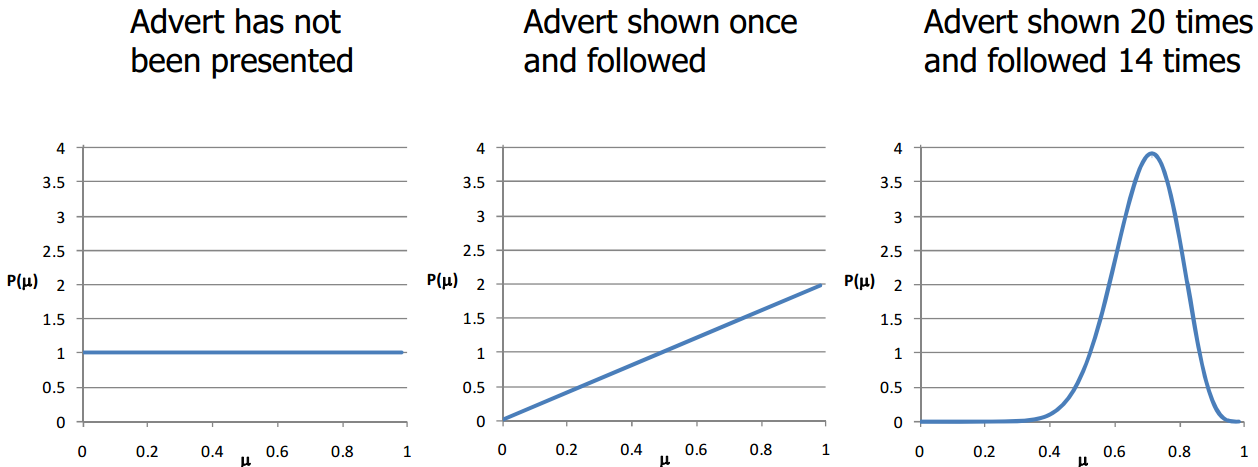
\includegraphics[width=\textwidth]{images/mu-graph.png}
%    \end{center}
    
%    Where $p(\mu)$ is defined thus;
%    $$ p(\mu) = \mu^t(1-\mu)^f $$

%    Where $t$ represents the number of true samples collected, and $f$, the number of false. As the size of $t+f$ grows, so too will the difference between the highest point on the distribution and the lowest, representing an increase in confidence. Note that this is a probability distribution of a continuous random variable, thus the area under the graph will sum to one.

\section{Collaborative Filtering}
    
    A method by which Amazon might decide Tim wants to buy Nerf blasters, HDMI adapters, bushcraft knives and sterling silver jewellery. Which he does. So it works.
    
    We have a set of products, $P$, a set of customers, $C$, and a sequence of shopping baskets, $B = (b_c)_{c\in C}$, all of which are described by vectors. Each shopping basket is a vector in $\{0,1\}^{|P|}$, with $b_{cp} = 1$ iff customer $c$ bought product $p$. Each shopping basket vector points in a direction which represents the products they've bought. Baskets which point in similar directions contain similar items. We define this similarity by using the cosine of the angles between the two vectors;
    
    \begin{equation}
        cos(\mathbf{x},\mathbf{y}) = \frac{\mathbf{x}\cdot\mathbf{y}}{||\mathbf{x}|| ||\mathbf{y}||}
    \end{equation}

    If the two vectors point in the same direction, the cosine will be 1. If they are perpendicular, the cosine will be 0. A collaborative Filter recommends the items in the baskets which points in the most similar direction to the baskets that the user has purchased, that is, if a user buys basket $\beta$, then we recommend the items in basket $b$ satisfying;
    
    $$
        b = \argmax_{b' \in B, b' \neq \beta} \frac{b'\cdot\beta}{||b'|| ||\beta||}
    $$

    We require that $b' \neq \beta$ (i.e cosine < 1), since whilst identical shopping baskets will point in identical directions, recommending that a customer buy items that he has already bought makes you look like an idiot.
    
    Collaborative filtering tends to give fairly good results in practical situations, but computing all those cosines is $O(|C||P|)$. To use some more technical terminology - it's really bloody slow.
    
    \subsection{Item to Item Collaborative Filtering}
        To resolve these performance issues, rather than calculating a customer's similarity to other customers, we can calculate items similarity. This approach allows for the offline pre-calculation based on existing data. This is the system Amazon uses, apparently. The formula for computing similarity stays the same, but we now compute every checked out basket containing one item with each basket containing the other, which is ($O(P^2)$). To aid in understanding, you can imagine each purchase as a row in a table; the columns represent all the products that we sell, and the values in the columns indicate whether that customer (row) has bought that item in their basket. In normal collab. filtering, we are comparing a new against other rows, which has to be computed for every new row. In Item-to-Item, we compare columns against columns, and recommend items with a high similarity to those in the customer's new basket.        
    
    \subsection{Association Rules}
    These are boolean-style IF-THEN combinations that recommend specific sets of additional items, based on a specific combination of inputs in the IF clause. For example, if we are selling Nerf guns, HDMI Adapters, Bushcraft Knives and Sterling Silver Jewellery, we might have a rule like this:
    \begin{center}
        IF NerfGun \^ BushcraftKnife THEN Jewellery\footnote{Well, it's not the recommendation I would make, but hey.}
    \end{center}
    In this system, if some shopper (let's call him, say, Tim), buys a nerf gun and a bushcraft knife then we will also recommend jewellery.
    
    Rules of this type have two metrics that we use to judge them: coverage and accuracy.
    \begin{itemize}
        \item Coverage: this is simply how many correct examples the rule applies to i.e how many Tims bought all three things.
        \item Accuracy: this is the coverage divided by the total number of samples that match the IF clause. I.e. the coverage divided by how many Tims bought Nerf guns and bushcraft knives.
    
    \end{itemize}
    We generate rules by listing all item sets from size 2 to size N, where N is any number we like. Typically smaller than the average basket size though. We also decide what minimum coverage/accuracy we will accept for our rules.
    
    Then we calculate the coverage of these sets (assuming no THEN part, this form of coverage just means how many baskets contain all items in the set), and discard those below a threshold we choose.
    
    Having done this, we go through each item set and create IF-THEN rules for each permutation of the items in it, only keeping the rules that satisfy the coverage and/or accuracy criteria that we want. We can evaluate the performance of our rulesets, or any classifier for that matter, with PRECISION and RECALL. Oh, what's that reader? You haven't heard those terms? FEAR NOT! JUST KEEP READING!
    \subsection{Precision and Recall}
    
    The precision of a recommendation system is the proportion of returned results which are relevant. The recall of a recommendation system is the proportion of relevant results which are returned.
    
    % Matt: I find this easier to digest:
    Another way to put it: precision represents "out of all the things I recommended, how many did they buy?", and recall represents "out of all the things they bought, how many did I recommend?"
    
    Consider two search engines, Bung and Wukupadua, or $B$ and $W$. On any given search, $B$ will return every single web page on the Internet, and $W$ will return exactly one page, which is definitely relevant to the subject matter.
    
    $B$ has a very high recall -- it will definitely return all relevant pages -- but it has a very low precision -- the vast majority of the web pages it returns are completely irrelevant.
    
    $W$ has a very low recall -- it will only return one of the many thousands of web pages on a particular subject -- but has a very high precision -- all of the results it returns are relevant.
    
    To give a more concrete example, my curent Amazon recommendations contain Bioshock: Infinite, Crysis 3, Bioshock and Metro: Last Light. I have just bought Bioshock Infinite and Sanctum 2 \footnote{Yes, I know, Sanctum is only on Steam. Shut up.}. Of the 4 recommendations 1 was relevant, so the precision is $\frac{1}{4}$. Of my 2 relevant purchases, 1 was recommended, so the recall is $\frac{1}{2}$.
    
\section{Decision Trees}
    Decision Trees are a machine learning algorithm based on binary trees. When categorising an item with a decision tree, we begin our ``journey'' at the root node. Each node prior to a leaf node specifies an attribute whose value enables our decision. Each branch from these nodes states an expected attribute value or condition, which we follow if our item meets the criteria. We repeat this process till we arrive at a leaf node, which categorises our item.
    
    An optimal decision tree is one in which at each transition down a level, the maximum information is gained. I like to think of it like a game of ``Guess Who''; at every round, we ask the broadest question possible eliminating as many options as possible. Only at the very end do we consider detailed characteristics.
    
    Decision trees are very prone to over-fitting, in that an unpruned decision tree made for a certain training dataset will perfectly classify \emph{that set} (achieve a 0 error rate). However, it is unlikely to perform as well on a test dataset as a tree pruned to some reasonable information gain, due to the high likelihood of noisy data in the training set.
    
    ``If two theories explain the facts equally well, then the simpler theory is to be preferred''. This principle is known as \emph{Occam's Razor}, but has little to do with shaving\footnote{There's a Treebeard joke in there somewhere but I'll be damned if I can find it.\footnote{YOU WHAT MATE??!?}}. The reason for this is while it is unlikely that a simple hypothesis fits the dataset by chance, it is comparatively likely that a complex one fits by chance, simply because there are so many more complex theories than simple ones.
    
    \subsection{Information Gain}
        So how do we calculate the ``maximum information gaining'' attribute? First consider what information gaining is; a reduction in entropy (our uncertainty in a r.v., in this case the item to be categorised). Clearly knowing the value of the attribute giving the most entropy will yield the maximum information gain. 
        
        We can therefore describe information gained from a training set $T$, knowing an attribute $a$, by calculating the entropy at our current node, then subtracting the entropy of each leaf node:
        
         $$ IG(T,a) = E(T) - E(T|a) $$

        Where $E$ denotes the entropy, which is defined as:
        
        $$ E(T) = -\sum\limits_{c} p_c \log_2p_c $$
        
        Where $p_c$ denotes the fraction of examples from class $c$.
        
    \subsection{Case Study: Microsoft Kinect}
        \emph{Note: This has come up in previous exams so is indeed worth knowing as a case study.}
        
        The Kinect uses decision trees to classify which pixels belong to which body parts in its field of vision. Training was done with a huge dataset (900,000 images) of \emph{rendered} human bodies. The genius of this approach is that, once a human body has been modelled, rigged, and its body parts labelled, it is trivial to render arbitrarily large sets of images of the body in different positions. It was therefore possible for Microsoft to completely fabricate their training set, avoiding painful hand labelling of real training data, which is unusual in machine learning.
        \emph{Jack has offered to clarify/add some stuff here}

\section{Back Propagation Neural Networks}
    Back propagation is a method of training neural networks. From a desired output, the network learns from many inputs, similar to the way a child learns to identify a dog from examples of dogs. We don't think the exact method will be examinable. If it is, then we'll also be stumped.


\end{document}
